\documentclass[a4paper,11pt]{article}
\usepackage{a4wide,graphicx,amsmath,amssymb,amsthm, algpseudocode, algorithm}
\usepackage[ruled, noline, algo2e, noend]{algorithm2e}
\usepackage{enumitem}
\usepackage{longtable}
\usepackage{array}
\usepackage{hyperref,url,color}
%\urlstyle{rm}

%----------------------- Macros and Definitions --------------------------

\newcommand{\N}{\ensuremath{\mathbb{N}}}
\newcommand{\R}{\ensuremath{\mathbb{R}}}
\newcommand{\Z}{\ensuremath{\mathbb{Z}}}
\newcommand{\M}{\ensuremath{\mathcal{M}}}

\graphicspath{{./images/}}

%-------------------------------- Title ----------------------------------

\title{Report Autonomous Vehicles and AI\\[1ex]
%
\large Autonomous Vehicles and Artificial Intelligence Lab}

\author{
    K. L. \\
    \and
    N. O. \\
    \and
    J. D. \\
    \and
    A. A.
}
\date{\today}

%--------------------------------- Text ----------------------------------

\begin{document}
\maketitle
\newpage
\tableofcontents
\newpage

\section{Introduction}

The F1Tenth car platform is a project for a small model race car and implements basic functionality like driving and steering. 
It also already comes with all the nodes required to fetch and publish sensor and transform data.\\
\newline
The developers provide manuals to build the hardware of the car platform and a software stack to interact with the basic components like steering, acceleration and the sensors. All of this is already implemented by the university staff and the interface is documented on the GitHub Repository of the F110 team.
In order to make it available in Gazebo Fortress we needed to implement an SDF file that implements the F110 standard in order for the simulation to be as close as possible to the real-world car platform.
The F110 car platform comes a 4-wheel drive, steering, IMU sensor, depth camera, RGB-camera and a LiDAR sensor.

\section{Expectations}
The goal of the project is the development of an autonomous race car capable of completing at least one lap on an indoor track in a fast yet safe manner.
The vehicle is positioned in the driving direction at the start. The race environment follows the F1TENTH cone system, where blue cones mark the left boundary, yellow cones mark the right boundary, and the start zone is identified by orange cones on both sides.
The track is a closed-loop circuit without any branches, and its layout changes between races. The vehicle operates without other cars on the track, with a maximum speed of approximately 15 km/h. 
A perception round precedes the timed lap. The system utilizes ROS2 Humble for software integration and runs on an NVIDIA Jetson NX 16GB. The vehicle is equipped with a 3D + mono depth camera (Intel RealSense Depth Camera D435i) and a high-resolution 2D LiDAR (Hokuyo UST-10), and features a four-wheel-drive system with Ackermann steering for navigation. \\
\newline
For this goal to be fulfilled, we assumed following elements to be given:
\newline
\begin{itemize}
	\item \textbf{Working hard- \& software stack}: In order to work effectively on this project, we assume that the given hard- and software stack is working as intended. 
	\item \textbf{Reliable WiFi connection to the car}: We need a reliable wireless connection to the car platform if we want to test it in the real world and also for the race. We assume that an SSH connection to the car with good data transfer speeds and little to none disconnections is possible.
	\item \textbf{Guidance \& support for debugging \& working with ROS2 Humble}: As we are no professionals regarding working with ROS2 and as debugging with ROS2 can be a complex task, we assume that we receive some more professional help with working with and especially debugging in ROS2.
\end{itemize}

\subsection{Functional Requirements}

The functional requirements describe what tasks the car should fulfil for driving autonomously. In the following table the main driving tasks (Perception, Localization, Mapping, Planning, and Control) are broken down into requirements fit to our project goals. Additionally, we introduced requirements for vehicle health and monitoring.

\begin{center}
	\begin{longtable}{ | m{2em} | m{10em} | m{16em} | m{8em} | }
		\caption{Functional Requirements.} \label{tab:long}\\
		
		\hline \multicolumn{1}{|m{2em}|}{\textbf{ID}} & \multicolumn{1}{m{10em}|}{\textbf{Requirement Name}} & \multicolumn{1}{m{16em}|}{\textbf{Requirement}} & \multicolumn{1}{m{8em}|}{\textbf{Classification}} \\ \hline
		\endfirsthead
		
		\multicolumn{4}{m{36em}}%
		{{\bfseries \tablename\ \thetable{} -- continued from previous page}} \\
		\hline \multicolumn{1}{|m{2em}|}{\textbf{ID}} & \multicolumn{1}{m{10em}|}{\textbf{Requirement Name}} & \multicolumn{1}{m{16em}|}{\textbf{Requirement}} & \multicolumn{1}{m{8em}|}{\textbf{Classification}} \\ \hline
		\endhead
		
		\hline \multicolumn{4}{|m{36em}|}{Continued on next page} \\ \hline
		\endfoot
		
		\hline \hline
		\endlastfoot
		
		F01 & General Perception & The vehicle shall capture real-time 3D depth data using the Hokuyo UST-10 LiDAR and high-resolution visual data using the Intel RealSense Depth Camera D435i to perceive the environment. & Must have\\
		\hline
		F02 & Object Detection \& Classification & The system shall detect and classify blue cones marking the left track boundary and yellow cones marking the right track boundary in real-time. & Must have\\
		\hline
		F03 & Cone Detection & When on track, the vehicle shall detect cones marking the track boundaries in real-time using the camera and LiDAR sensors. & Must have\\
		\hline
		F04 & Sensor Fusion & When collecting data, the perception system shall integrate LiDAR and camera data using a sensor fusion algorithm to improve cone detection accuracy. & Must have\\
		\hline
		F05 & Distance Estimation & While driving, the vehicle shall estimate the distance to the track boundaries continuously. & Should have\\
		\hline
		F06 & Point Cloud & The vehicle shall collect 3D LiDAR point cloud data to detect and map its surroundings in real-time. & Must have\\
		\hline
		F07 & Visual Data & The camera system shall provide input for visual odometry and SLAM, ensuring accurate self-localization. & Should have\\
		\hline
		F08 & Self-Localization & The vehicle shall localize its position relative to track boundaries using fused data from LiDAR, camera, and odometry. & Must have\\
		\hline
		F09 & Real-Time Map & The vehicle shall generate a real-time map of the environment using LiDAR and visual sensors, aiding in cone detection and path planning. & Must have\\
		\hline
		F10 & Environments & The system shall be able to handle both static and dynamic environments, where the track layout may change. & Could have\\
		\hline
		F11 & Optimal Trajectory & When planning the path, the vehicle shall generate an optimal trajectory within track boundaries using the detected cone positions and real-time sensor data, maintaining the desired speed. & Should have\\
		\hline
		F12 & Path Planning & The vehicle shall implement a planning algorithm that works in real time, adjusting paths as the environment changes. & Could have\\
		\hline
		F13 & Path Updates & The path planner shall compute new trajectories dynamically to handle sudden track changes. & Could have\\
		\hline
		F14 & Acceleration \& Deceleration & The vehicle shall decide when to accelerate, decelerate, or stop, depending on the environment. & Should have\\
		\hline
		F15 & Driving Modes & The vehicle shall be able to switch between different driving modes (e.g., cruising, emergency stop) based on the context. & Should have\\
		\hline
		F16 & Speed Maintenance & The vehicle shall maintain the fastest appropriate speed for the calculated paths on the track layout, not exceeding 15 km/h. & Should have\\
		\hline
		F17 & Acceleration Adaptation & The system shall adapt acceleration to keep the vehicle within speed limits, adjusting for factors like road slope, friction, and other dynamic conditions. & Could have\\
		\hline
		F18 & Sharp Turns & While approaching sharp turns, the vehicle shall adjust its speed to ensure safe cornering without exceeding the track boundaries. & Should have\\
		\hline
		F19 & Smooth Acceleration & When accelerating, the vehicle must limit its acceleration to avoid jerky movements using a soft acceleration curve, ensuring smooth control. & Should have\\
		\hline
		F20 & Braking & The vehicle shall be able to brake in real-time to slow down or stop based on planned behavior or unexpected events. & Could have\\
		\hline
		F21 & Controlled Emergency Braking & When braking, the vehicle shall decelerate within a controlled distance to avoid overshooting turns or track boundaries. & Could have\\
		\hline
		F22 & Steering Angle & When controlling the steering, the vehicle shall calculate the optimal steering angle based on the track curvature and current speed. & Must have\\
		\hline
		F23 & Steering & The vehicle shall control the Ackerman steering system to follow the planned trajectory accurately. & Must have\\
		\hline
		F24 & Smooth Steering & The control system shall ensure stable and smooth steering, especially at high speeds. & Should have\\
		\hline
		F25 & External Signals & The system shall respond appropriately to external signals and traffic rules defined for the track. & Could have\\
		\hline
		F26 & Failsafe Mode & When a critical system failure is detected, the vehicle shall engage the emergency braking system to bring the vehicle to a stop. & Should have\\
		\hline
		F27 & System Health & When system health is checked, the vehicle shall monitor the status of all sensors, compute hardware, and actuators in real-time to ensure continuous operation. & Could have \\
		\hline
		F28 & Odometry & The vehicle shall collect odometry data to track its speed, orientation, and position over time. & Must have\\
		\hline
		F29 & Health Checks & The system shall implement watchdog timers and health-check nodes to detect failures or malfunctions in any part of the system. & Should have\\
		\hline
		F30 & Vehicle Tracking & The system shall provide continuous and real-time feedback on the vehicle's movement and position to maintain trajectory tracking. & Must have \\
		\hline
		F31 & Internal Communication & All sensors, actuators, and the onboard compute hardware shall communicate via ROS2 Humble, using DDS for real-time message passing. & Must have\\
		\hline
		F32 & Manual Override Mode & The system should be able to transition to a manual override mode in case of critical failures, allowing the race team to take control if necessary. & Should have\\
		\hline
		F33 & Partial System Failures & The system shall include multiple levels of safety checks, and emergency overrides shall be functional even in the event of partial system failures. & Should have\\
		\hline
		F34 & Testing & The vehicle shall be tested in both simulation and real-world environments to validate its perception, planning, and control systems. & Should have \\
		\hline
	\end{longtable}
\end{center}

\subsection{Quality Requirements}

The quality requirements ensure that the car is working within its constraints as intended. Furthermore some quality requirements are requirements towards the hardware and some numerical values may differ in the end depending on average and maximum speeds achieved by the racecar in the final implementation.

\begin{center}
	\begin{longtable}{ | m{2em} | m{10em} | m{16em} | m{8em} | }
		\caption{Quality Requirements.} \label{tab:long}\\
		
		\hline \multicolumn{1}{|m{2em}|}{\textbf{ID}} & \multicolumn{1}{m{10em}|}{\textbf{Requirement Name}} & \multicolumn{1}{m{16em}|}{\textbf{Requirement}} & \multicolumn{1}{m{8em}|}{\textbf{Classification}} \\ \hline
		\endfirsthead
		
		\multicolumn{4}{m{36em}}%
		{{\bfseries \tablename\ \thetable{} -- continued from previous page}} \\
		\hline \multicolumn{1}{|m{2em}|}{\textbf{ID}} & \multicolumn{1}{m{10em}|}{\textbf{Requirement Name}} & \multicolumn{1}{m{16em}|}{\textbf{Requirement}} & \multicolumn{1}{m{8em}|}{\textbf{Classification}} \\ \hline
		\endhead
		
		\hline \multicolumn{4}{|m{36em}|}{Continued on next page} \\ \hline
		\endfoot
		
		\hline \hline
		\endlastfoot
		
		Q01 & Sensor Processing Latency & The system shall process sensor data in real-time with latency under 50 ms to ensure timely decision-making and control. & Must have \\
		\hline
		Q02 & Control Loop Frequency & The vehicle shall maintain a control loop update frequency of 20-30 Hz to ensure smooth and responsive driving at max. 15 km/h. & Must have \\
		\hline
		Q03 & Localization Accuracy & The localization system shall maintain its position estimation with an accuracy \(\pm 10\) cm to ensure the vehicle stays within the track boundaries. & Should have \\
		\hline
		Q04 & Perception Radius & The perception system shall detect cones at least 10 meters ahead to provide sufficient time for path adjustments. & Must have \\
		\hline
		Q05 & Emergency Braking Distance & The vehicle shall decelerate within 2-3 meters when the emergency braking system is engaged to ensure safe stopping. & Must have \\
		\hline
		Q06 & Emergency Stop & The vehicle shall engage the emergency braking system within 100 ms of detecting critical system failures to avoid accidents. & Should have \\
		\hline
		Q07 & Detection Rate & The perception system shall maintain a continuous detection rate of at least 95\% for cones to prevent boundary violations. & Must have \\
		\hline
		Q08 & Detection \& Classification Range & The system shall detect and classify blue cones marking the left track boundary and yellow cones marking the right track boundary in real-time within a range of at least 2 m. & Must have \\
		\hline
		Q9 & Control System & The control system shall operate continuously for the duration of the race without any system crashes or interruptions. & Should have \\
		\hline
		Q10 & Fallback & The vehicle shall recover from sensor or communication failures within 200 ms using fallback systems to ensure continuous operation. & Could have \\
		\hline
		Q11 & Logs & The system shall log sensor and control data with timestamps for a post-race analysis without exceeding storage limits. & Should have \\
		\hline
		Q12 & Hardware Temperature & The compute hardware shall maintain stable operation within a temperature range of 0-50°C to prevent overheating or shutdowns. & Could have \\
		\hline
		Q13 & Real-Time Data & The system shall provide real-time telemetry data to the race team at least once every 100 ms to allow for remote monitoring during the race. & Should have \\
		\hline
		Q14 & Reconfiguration \& Updates & The system shall support easy reconfiguration and updates of perception and control algorithms without requiring major code overhauls. & Could have \\
		\hline
		Q15 & Diagnostics & The user interface shall allow for quick diagnostic checks of system health before and during the race to facilitate rapid troubleshooting. & Could have \\
		\hline
		Q16 & Real-Time Internal Communication & The system shall support reliable, low-latency communication between sensor nodes, perception nodes, and control nodes to ensure real-time response. & Must have \\
		\hline
		Q17 & Energy Consumption & The software stack should optimize CPU and GPU usage to minimize energy consumption during intensive tasks like real-time perception and path planning. & Should have \\
		\hline
		Q18 & Sensor Efficiency & The vehicle shall use its sensors efficiently, ensuring that data redundancy is minimized, and sensor processing loads are balances to avoid system bottlenecks. & Must have \\
		\hline
		Q19 & Data Filtering & The system should implement intelligent data filtering to reduce unnecessary sensor data while preserving critical information needed for accurate perception and planning. & Must have \\
		\hline
		Q20 & Trajectory Updates & The path planning system shall generate new trajectories within a strict time frame/ every 50 ms to adapt to changes in the environment, avoiding delays that could cause the vehicle to miss turns. & Must have 
	\end{longtable}
\end{center}


\subsection{Constraints}

The constraints are defined by the limitations of the hardware and the rules of the Formula Student Driverless. They limit our solution space in order to yield a feasible solution in the end.

\begin{center}
	\begin{longtable}{ | m{2em} | m{10em} | m{16em} | m{8em} | }
		\caption{Constraints.} \label{tab:long}\\
		
		\hline \multicolumn{1}{|m{2em}|}{\textbf{ID}} & \multicolumn{1}{m{10em}|}{\textbf{Requirement Name}} & \multicolumn{1}{m{16em}|}{\textbf{Requirement}} & \multicolumn{1}{m{8em}|}{\textbf{Classification}} \\ \hline
		\endfirsthead
		
		\multicolumn{4}{m{36em}}%
		{{\bfseries \tablename\ \thetable{} -- continued from previous page}} \\
		\hline \multicolumn{1}{|m{2em}|}{\textbf{ID}} & \multicolumn{1}{m{10em}|}{\textbf{Requirement Name}} & \multicolumn{1}{m{16em}|}{\textbf{Requirement}} & \multicolumn{1}{m{8em}|}{\textbf{Classification}} \\ \hline
		\endhead
		
		\hline \multicolumn{4}{|m{36em}|}{Continued on next page} \\ \hline
		\endfoot
		
		\hline \hline
		\endlastfoot
		
		C01 & Speed Limit & The vehicle shall not exceed a speed of 15 km/h due to track limitations and safety considerations. & Must have \\
		\hline
		C02 & Jetson Limitations & The system shall operate within the limitations of the NVIDIA Jetson NX ensuring all processes can run in real-time without overloading the CPU, GPU, and memory resources. & Must have \\
		\hline
		C03 & Real-Time Performance & The system shall process sensor inputs at 20-30Hz to maintain real-time performance within the computational limits of the vehicle. & Should have \\
		\hline
		C04 & Remote Emergency Stop & The vehicle shall include a Remote Emergency Stop system that can be triggered by the race team/ race officials at any time during the race. & Should have \\
		\hline
		C05 & System Monitoring & The autonomous system shall continuously monitor critical safety components and transition to a safe state if a failure is detected. & Should have \\
		\hline
		C06 & Power Budget & The sensor suite shall operate within a power budget, ensuring no component exceeds the power capacity available to the vehicle. & Should have \\
		\hline
		C07 & Ackerman Steering & The vehicle shall use the Ackerman steering system for turning, which constrains the types of maneuvers the vehicle can perform, preventing mechanical failure or loss of control, especially at high speeds. & Must have \\
		\hline
		C08 & On Track Testing & Vehicle testing on track shall be done within the practice tracks provided. & Should have \\
		\hline
		C09 & Processor Limitations & Algorithms for perception, planning, and control shall be designed to avoid overloading the processor, ensuring real-time performance without exceeding the power and thermal limits of the hardware. & Must have \\
		\hline
		C10 & 4-Wheel Drive & The vehicle's control system shall optimize the distribution of torque across all four wheels in a manner that ensures both optimal acceleration and stability, without causing skidding or loss of traction. & Should have \\
		\hline
		C11 & Energy Consumption & The vehicle's energy consumption shall be managed to ensure that it can complete the entire race or testing session within the available battery capacity, taking into account the energy demands of high-speed racing and intensive computations. & Must have \\
		\hline
		C12 & Data Prioritization & The system shall ensure that critical sensor data is prioritized in high-speed scenarios, where rapid decision-making is essential. & Should have \\
		\hline
		
	\end{longtable}
\end{center}




\section{Architecture}
\begin{figure}[H]
\begin{center}
\centerline{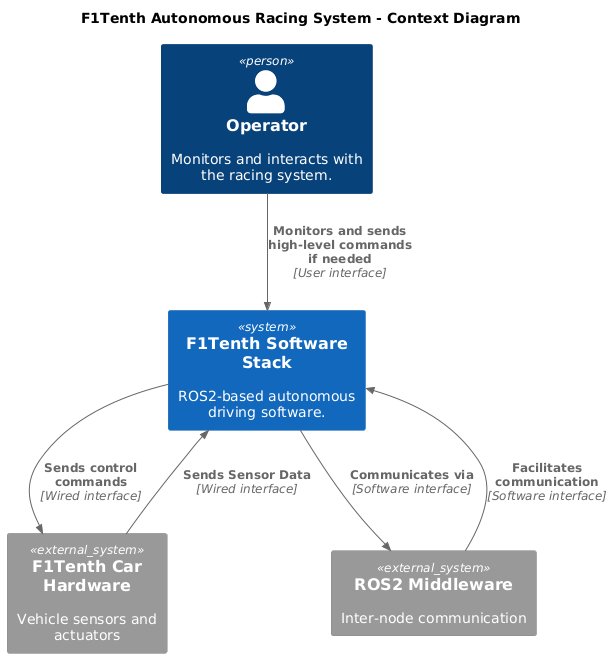
\includegraphics[width=\columnwidth]{Context.png}}
\caption{Context diagram (C4 Level 1) of the used software architecture}
\label{fig:arch-context}
\end{center}
\end{figure}
The software architecture is based on a software stack which uses the ROS2 Middleware to facilitate communication and sends drive commands to as well as receives sensor data from a provided F1Tenth Hardware Stack as seen in Figure~\ref{fig:arch-context}.
\begin{figure}[H]
\begin{center}
\centerline{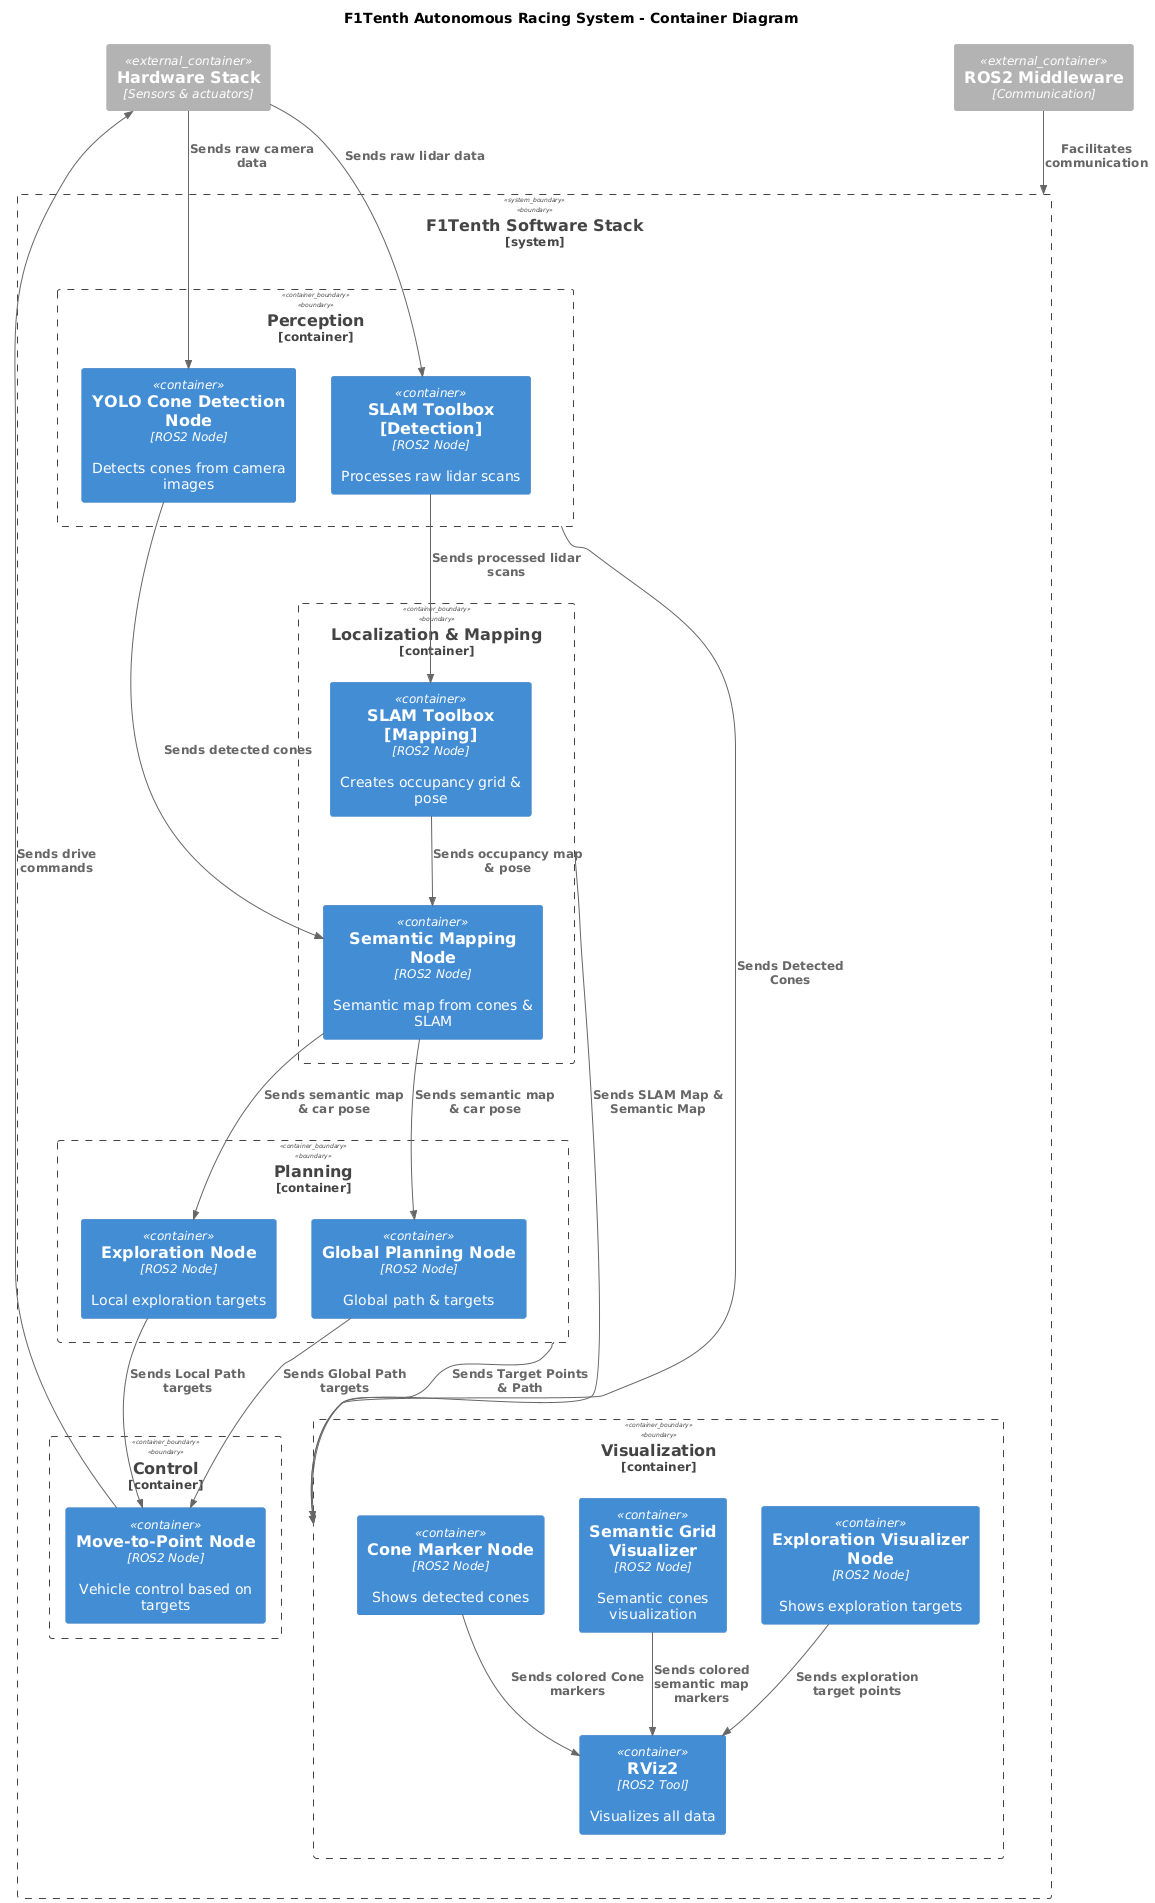
\includegraphics[width=0.85\columnwidth]{Container.png}}
\caption{Container diagram (C4 Level 2) of the used software architecture}
\label{fig:arch-container}
\end{center}
\end{figure}
As shown in Figure~\ref{fig:arch-container}, the autonomous vehicle system is divided into several interconnected modules that ensure efficient perception, localization \& mapping, planning and control. 
The perception system includes cone detection, which is performed by a YOLO-based node that uses a trained deep learning model to identify cones in the camera image.
Here, SLAM Toolbox is used to interpret the LIDAR sensor data.
\newline
In the localization \& mapping module, the LIDAR-based map and corrected pose information from the SLAM Toolbox, as well as the cone detections from the perception module are fused in a Semantic Mapping Node. The resulting semantic map, which now includes cone color information is essential for the path planning. 
\newline
The path planning module generates an optimal trajectory that ensures that the vehicle navigates the track efficiently. It processes environmental information, vehicle dynamics, and track constraints to determine a feasible and optimized driving path.
The planning process consists of two stages. Initially, the system explores the track to gather key information about the environment and construct a representation of the drivable space. Once sufficient data is collected, the module transitions to a global planning mode, where it optimizes the trajectory based on the recorded driving path to ensure smooth navigation.
\newline
Target points calculated by the planning module are sent to the control module to be further processed into drive commands for our hardware stack.
\newline
Additionally, a visualization module gets intermittent outputs from each module to visualize calculated perception detections, maps and paths via RViz2.\\

\section{Simulation}
In order to quickly iterate, work in parallel, and also work independently from the racecar on the project a simulation was implemented using Gazebo Fortress as a simulator.
Gazebo is a lightweight simulator which implements the SDF file format to describe robots and worlds and has close integrations with ROS2.
Since the project is constrained to using ROS2 Humble, the Fortress version was chosen since it is the recommended platform for Humble and Ubuntu jammy.
For the LiDAR sensor the Gazebo implementation is used and parametrized to fit the properties of the Sick LiDAR used by the F1Tenth hardware.
The RGB- and depth camera is modelled using the \textbf{TODO}.

\subsection{Gazebo Communication}

Even though Gazebo Fortress is still under long-term-support (LTS) it does not come with python bindings for the Gazebo transport layer. 
This layer would usually handle all communication with the simulation using sockets and is available in newer version of Gazebo (like Ionic). 
However Gazebo Fortress exposes services over a CLI. This can be used to implement the Gazebo message-protocol using system calls which can then be executed using python. 
The whole implementation is available in the Github repository of this project and implements the different message types using the pydantic framework. 
The messages are then serialized into strings and sent to Gazebo over a system call. 
Even though some service calls can be batched for example when spawning many entities (cones) at once, 
this approach introduces some delays and the system calls can also timeout when send with a high frequency.\\
\newline
The main services made available this way are:

\begin{itemize}
\item "/world/:world:/create"
\item "/world/:world:/create\_multiple"
\item "/world/:world:/set\_pose"
\item "/world/:world:/remove"
\item "/world/:world:/control"
\end{itemize}


The \textbf{create} service can be used to instantiate SDF-files into a running Gazebo simulation where the models are instantiated as a blocking call (appear immediately from the perspective of the simulation). \textbf{create\_multiple} can be used to batch many calls to the create service to reduce the load. \textbf{set\_pose} is a service for manipulating the position and rotation of entities in the simulation. In this project it is used to set the position and rotation of the vehicle to a neutral position after a reset call to the environment.\\
The \textbf{remove} service can be used to remove entities from the simulation. This call can unfortunately not be batched resulting in very long execution times when trying to remove many entities from the simulation. At first this was supposed to generate a new track every time the environment was reset but the associated rebuild time resulted in infeasible training times (over a minute for a rebuild).\\
\textbf{control} is a service able to start or stop the simulation or run it for a certain amount of time steps. This was first used to make the `step` function of the environment deterministic but resulted in too many system calls for Gazebo which resulted in data inconsistencies and dropped calls.

\subsection{Environment Generation}

Since the Formula Student tracks are defined by cones we implemented a generator for tracks with some free parameters like size, width, cone distance and shape.
The track generation algorithm samples $n$-points from a normal distribution $\mathcal{N}(\mu, \sigma^2)$ with $\mu = 0$ and $\sigma = 1$ to create a 2D point cloud. These points are then used to calculate the concave hull to retrieve the outer shape of the point cloud. At first I tried using the convex-hull of the point cloud but a concave-hull does not contain left-curves (when traversed clock-wise) which would truncate the action space by half since only positive steering angles would be required to traverse the track. This would lead to poor generalization when tested in the real world where tracks will contain left curves. The set of points of the concave hull is then z-normalized (subtraction of mean divided by the standard deviation) and then scaled to the desired track size.
Afterwards a polygon is created from the concave hull and buffered by the track width $w$ to produce an inner and outer polygon boundary defining the border of the track. The track can now still contain some sharp curves that are not fit for the car platform since it can not steer around them. To solve this, Chaikins corner cutting algorithm \cite{chaikin1974algorithm} was applied to the borders where the number of refinements $r$ is a free parameter.\\
\newline
The application of the corner cutting algorithm now leaves the borders of the track with sparse data points on straight sections and dense data points on the refined sections where sharp curves occurred. To end up with an even distribution of cone positions the borders are resampled using linear interpolation.
In order to introduce some more complex track environments, the $d$ parameter can be used to pull $d$ evenly spaced points from the concave hull inwards, leading to sharper curves.

\begin{algorithm}[tb]
\caption{Track Gen}
\label{alg:track-gen}
\begin{algorithmic}
\State {\bfseries Input:} $n$, $s_x$, $s_y$, $w$, $r$, $\alpha$, $d$
\State $X_n \sim \mathcal{N}(\mu,\,\sigma^{2})$
\State $C_0$ = alphaShape($X, \alpha$)
\State $C_0$ = applyDents($C_0, d$)
\State $C_\text{norm}$ = zNorm($C_0$)
\State C = stack($C_x \cdot s_x, C_y \cdot s_y$)
\State $T_\text{outer}$ = buffer($C_\text{norm}, w/2$)
\State $T_\text{inner}$ = buffer($C_\text{norm}, -w/2$)
\State $T_\text{router}$ = chaikin($T_\text{outer}, r$)
\State $T_\text{rinner}$ = chaikin($T_\text{inner}, r$)
\State $T_\text{souter}$ = resample($T_\text{router}$)
\State $T_\text{sinner}$ = resample($T_\text{rinnter}$)
\State {\bfseries Return:} $T_\text{souter}, T_\text{sinner}$
\end{algorithmic}
\end{algorithm}

Figure \ref{fig:track} shows the generated track for the environment from a top-down perspective. The blue dots describe the cone positions. The origin of the track is in the middle at the very top since the coordinate system in Gazebo uses the y-direction as a forward direction. The track is then traversed in clock-wise direction.

\begin{figure}[ht]
\vskip 0.2in
\begin{center}
\centerline{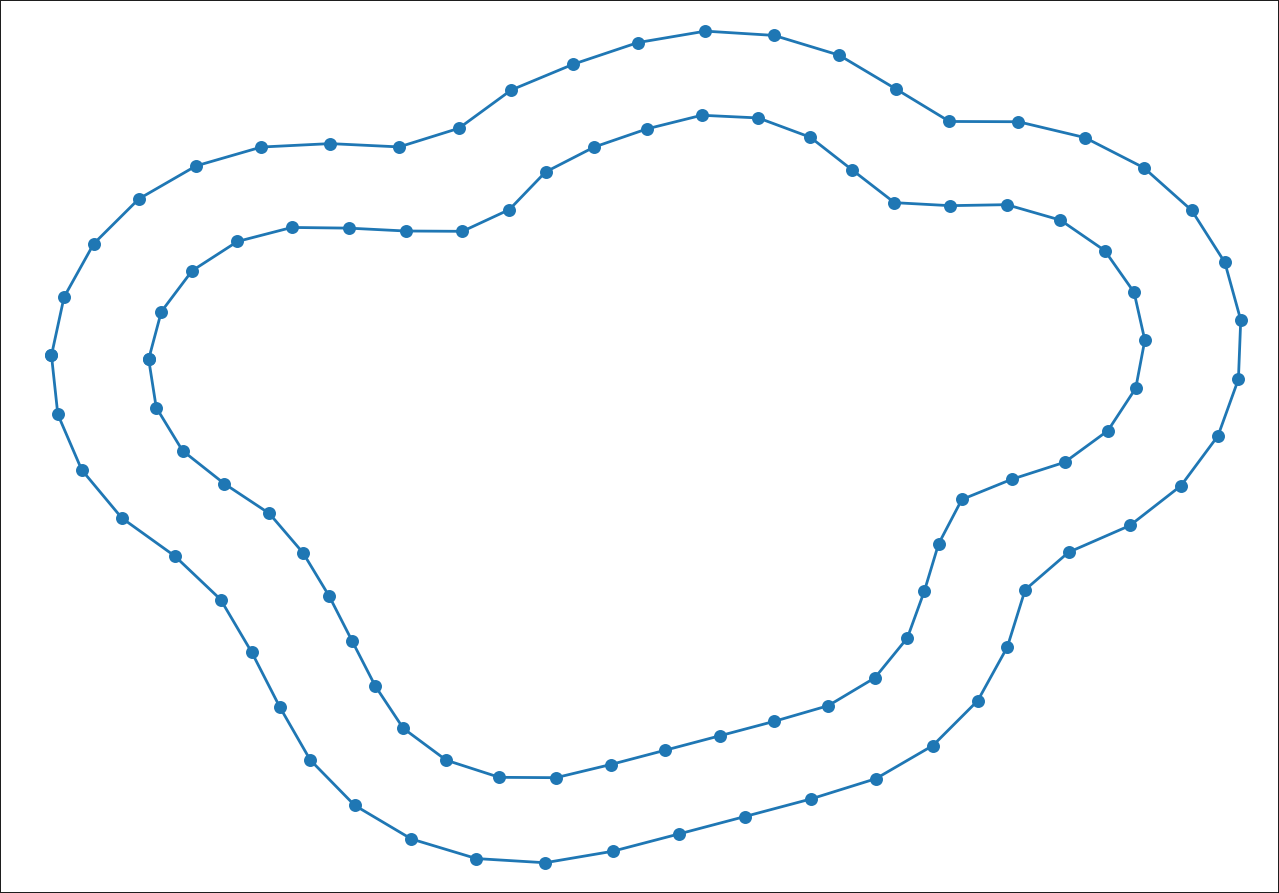
\includegraphics[width=\columnwidth]{track.png}}
\caption{The generated track boundaries using the RNG seed 42 with the parameters later used in training. Blue dots mark the positions of cones.}
\label{fig:track}
\end{center}
\vskip -0.2in
\end{figure}

\subsection{Gazebo ROS2 Communication}

Apart from system calls to interact with services provided by Gazebo Fortress we use the ROS-Gazebo-Bridge to convert the topics and data types published in Gazebo to ROS2. 
This is a transport layer that is available in python and can be launched using ROS2 and the regular python launch file syntax. 
This conversion process is very resource intensive which is why only the LiDAR sensor and the odometry can be updated with a high frequency.



\section{Implementation}
\textbf{TODO: Incorporate elements of the presentation into the text.} The whole implementation can be found in the GitHub 
\textbf{TODO: Link to repository!} repository. In this section we will show the purposes of each node implementation and how they are related to achieve the desired functionalities.


The implementation timeline was mostly usecase driven since our team did not have any practical experience with the ROS2 middleware and Gazebo Fortress as a simulator. Because of this we decided early on that we need a way to iterate over different implementations and test sensor feedback from the car platform. In order to get familiar with the ROS2 message formats and the implementation of ROS2 nodes in python using \textit{rclpy} as a dependency we implemented the \textit{wasd\_control} node. The node is located in the \textit{test\_package} of our ROS2 workspace. The package is utilized as a point in the project where ideas could be implemented and integrated quickly without interrupting the main stack. The control node acts as a keyboard controller for the ackermann steering system and gave us some insights of how the system needs to be updated in order to get a smooth driving behavior. The node implements a state machine that checks for keyboardThis was also the point in the project where we did face the delays that are introduced by the bad network connection available for the project. We experienced control delays from our machine to the vehicle of up to one second which is infeasible for a live feedback loop. This also limited our capabilities of creating visualizations since we had no way of sending them to our monitors since the network bandwidth was so low.


Because of this limitation and the only local availability of the vehicle we moved to implementing the simulation using Gazebo Fortress. In order to work with Gazebo Fortress we had to familiarize ourselves with the concept of modeling for a simulation and in what file format we want to define our models. Ultimately we chose the SDF file format since it is an open source format with relatively new and comprehensive documentation. The URDF and XACRO formats are mainly associated with ROS in the documentation which introduces a barrier, making it harder to work with. These file formats also separate aspects of the same model into different files. This reduces observability of connected components. Having everything in a single file format also reduces complexity since we only had to learn a single new format. In order to implement the vehicle platform and a world around it we heavily utilized the tutorials on the Gazebo documentation \cite{gazebo-documentation}. The first iteration of the vehicle platform was implemented using their \textit{Build your own robot} tutorial and later remodeled once we had a deeper understanding about the file formats and available plugins. At this stage in the development we were able to utilize the examples implemented in the \textit{gazebo\_tutorials} GitHub repository \cite{gazebo-tutorials}. From the repository we learned how to model the Gazebo UI using SDF files and how to implement the transform tree for our vehicle platform in order to have a better transfer to our ROS2 implementation. In the later stages of developing the simulation we focused on getting the data and structure of the messages as close to the real vehicle platform as possible. This was achieved using the ROS2-Gazebo-Bridge \cite{ros-gz-bridge}. With this bridge we could convert the Gazebo-messages to ROS2 messages and forward the topics to ROS2 as well as remap them to the correct paths if necessary. In the end the simulation was close to interchangeable with the implementation of the car platform and we could reuse our complete software stack in the launch files for Gazebo without heavy modifications.

Due to the theoretical knowledge we obtained from participating in the lecture about autonomous vehicles and artificial intelligence preceding this project our methodology was to implement the best practices we learned in the lecture. This involves a software architecture comprised of different modules that are responsible for subtasks of the overall driving task. The smallest module we could think of was the task of moving to a point in a given coordinate system. In order to achieve that we experimented with the odometry data coming from the drive controller of the simulation and the vesc module of the F1Tenth system stack. We noticed that the coordinate systems between ROS2 and Gazebo are different and started to implement the required logic using the coordinate system from Gazebo with the plan to implement logic to translate it to ROS2. The coordinate system in Gazebo uses the $y$-direction as forward direction and $-x$ as the direction to the right. In this stage of development the \textit{MoveToPoint} ROS2 node. This node receives a new target point using \textit{PoseStamped} messages. Once a target point has been received the node checks its current position using a pose it received from some odometry or SLAM (Simoultaneous Localization And Mapping) topic. From the current pose and the target point it calculates a steering angle using the difference in vehicle rotation and target point direction compared to the current vehicle position. This steering angle is of course clipped by the capabilities of the ackermann steering system but recalculated every time the node receives a new vehicle pose estimation, leading to a smooth steering towards the target point. Once a target point is reached, i.e. the distance to the target point is less than a parametrized $\epsilon$, the vehicle stops until it receives a new target point further away.
Figure \ref{fig:move-to-point} visualizes the calculation of the steering angle using the vehicle orientation and the target point. The red circle visualizes the $\epsilon$ distance below which the vehicle will stop approaching the target point.

\begin{figure}[ht]
\vskip 0.2in
\begin{center}
\centerline{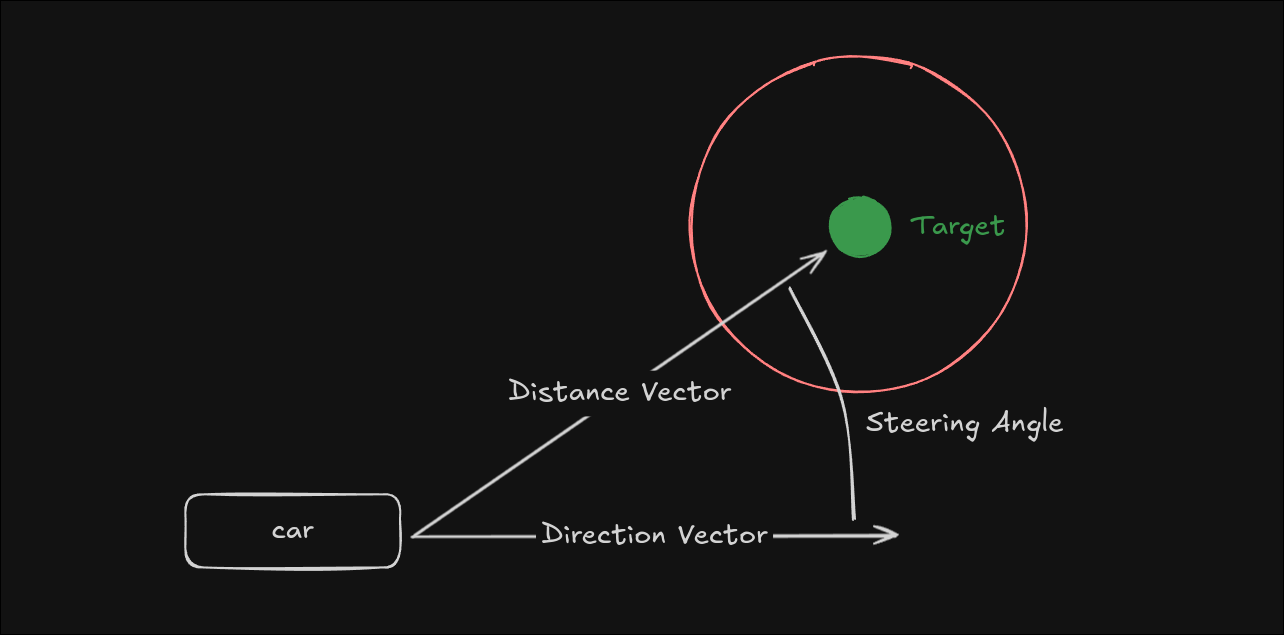
\includegraphics[width=\columnwidth]{move-to-point-vis.png}}
\caption{Schema of the inner workings of the \textit{MoveToPoint} ROS2 node. The figure displays the calculation of the steering angle using vehicle orientation and target point. The red circle marks the $\epsilon$ distance at which the vehicle will stop driving towards the point once inside.}
\label{fig:move-to-point}
\end{center}
\vskip -0.2in
\end{figure}

After iterating over the \textit{MoveToPoint} node we did notice that the coordinate system of ROS2 was in reality more different than expected which we solved using a custom transform at that time. Due to large drifts in the odometry data of the vehicle in the real world we looked into the next building block for our software stack which was SLAM. SLAM would solve the drifting odometry and provide us with the tools necessary to build a map of the environment that we could enhance with additional information from other sensor systems to create a global plan for driving. Implementing SLAM proved infeasible however since during our experiments we noticed that the transforms from the ROS2 transform tree applied to the sensor data used by the SLAM Toolbox yielded very bad results. The sensor data and map information was drifting a lot. The result was an unusable map and no information about even the immediate proximity of the vehicle. Because of this we tried to create a map without using readily available tools like the SLAM Toolbox which also turned out to be infeasible since the noise of the environment requires robust odometry (roboust meaning it drifts in acceptable margins) and elaborate algorithms that could track objects in the environment over multiple frames of sensor data.

Fortunately, after an update of the hardware stack, the transform problems experienced in the context of the SLAM Toolbox were resolved. With stable transforms, we successfully generated accurate maps using LIDAR data processed by the SLAM Toolbox, providing a reliable baseline map for our autonomous navigation tasks.
To further enhance our mapping and navigation capabilities, we integrated semantic information related to cones through a dedicated node, the \textbf{YoloConeDetectionNode}. This node utilizes a YOLO deep-learning model specifically trained on a provided dataset of cone images. The YOLO model facilitates accurate 3D detection of cones while also assigning semantic labels (e.g., the cone colors).
It performs the following key tasks:

\begin{enumerate}
    \item \textbf{2D Cone Detection}: It processes raw RGB images obtained from the Intel RealSense color camera, detecting cones and generating bounding boxes with associated semantic labels indicating the cone type (e.g., the color-based classification).

    \item \textbf{Depth-Based Localization}: To translate these 2D detections into accurate 3D positions relative to the robot, we perform an additional depth-based localization step using the depth information from the RealSense depth sensor, as well as the provided intrinsics and extrinsics from the depth to the color camera. Due to possible misalignments between RGB and depth sensors, direct pixel-to-pixel mapping between color and depth images is not straightforward. Thus, we use an approach analogous to the one used in the Intel RealSense SDK:
    
    \begin{itemize}
        \item \textit{Pixel Correspondence}: For each detected cone, the algorithm identifies the center pixel of its YOLO bounding box in the RGB image. This RGB pixel is then projected onto a corresponding pixel in the depth image through the following procedure:
        
        \begin{enumerate}[label=(\alph*)]
            \item \textbf{Projection to a 3D Line}: The algorithm first takes the RGB pixel coordinates and projects them into two hypothetical 3D points, one at the minimum depth ($depth_{min}$) and one at the maximum depth ($depth_{max}$) limits.
            
            \item \textbf{Image Transformation}: These two 3D points, originally defined in the color image, are transformed into the depth image using pre-calibrated extrinsic parameters.
            
            \item \textbf{Back-Projection to the Depth Image Plane}: The transformed points define a line segment in the depth image plane, representing possible correspondences of the original RGB pixel.
            
            \item \textbf{Optimal Pixel Selection}: The algorithm searches along this line segment in the depth image to find a pixel that, when re-projected into the RGB image, minimizes the distance (error) to the original RGB detection pixel. This step ensures robust and accurate alignment, effectively resolving intrinsic or extrinsic misalignment between sensors.
        \end{enumerate}
        
        \item \textit{Depth Value Extraction and Averaging}: After selecting the optimal depth pixel, the node computes a median depth value from a small pixel patch around it. This averaging further reduces the influence of noise and outliers.
        
    \end{itemize}

    \item \textbf{Transformation using ROS2 TF}: The resulting 3D coordinates are then transformed into the robot's coordinate frame (\texttt{base\_link}) using ROS2's TF2 transformations.
\end{enumerate}

The detected cones will be visualized in RViz via the \textbf{ConeMarkerNode}, which listens to a DetectedConeArray, transforms the cone positions into a target frame, and publishes visual markers to RViz.\\
\newline

The resulting 3D coordinates and their label information are then further used in a \textbf{SemanticMappingNode}, fusing the LIDAR-based map from the SLAM Toolbox with the detected labeled cones to create an occupancy map with semantic information for later use in our planning. The semantic mapping process works as follows:

\begin{enumerate}
    \item \textbf{SLAM Occupancy Grid Processing}:  
    The node subscribes to occupancy grid maps published by the SLAM Toolbox. Upon receiving a new map, it first filters out noise and irrelevant objects based on predefined model assumptions (e.g., maximum object length and minimum object area). This is achieved by identifying connected clusters of occupied grid cells and removing clusters that do not meet these criteria.

    \item \textbf{Cone Detections Integration}:  
    Detected cones from the YOLO-based cone detection node are received. Each cone’s position is transformed from its sensor frame into the global map coordinate frame using ROS2's TF2 transformations, ensuring alignment with the SLAM map and is then stored with a detection timestamp.

    \item \textbf{Semantic Labeling via Cluster Matching}:  
    The filtered occupancy grid is processed to identify connected clusters of occupied cells. Each cluster represents a potential object or obstacle. The algorithm calculates centroids for these clusters, stores them if they are new or matches them against a previously stored cluster, and then compares each centroid’s position against the transformed cones detections. If a cone detection is found within a predefined merge threshold distance, the cluster receives a "hit" corresponding to the cone's semantic label (e.g., cone color).

    Clusters store persistent semantic information by counting the number of hits per label. When assigning semantic labels, each cluster takes on the semantic label with the most hits, providing robust and stable labeling despite potential detection noise or sensor inaccuracies.

    \item \textbf{Semantic Grid Generation}:  
    Finally, a \texttt{SemanticGrid} message is created, containing occupancy information and semantic labels for each cell. Cells in each identified cluster inherit the cluster's dominant semantic label. This semantic map can be directly utilized by downstream exploration and planning modules.

    \item \textbf{Maintenance and Decay}:  
    Cone detections are timestamped and periodically purged based on a decay threshold or if they were already used in the labeling of a cluster. This ensures that outdated or already matched detections do not permanently influence the map’s semantics.

\end{enumerate}

The computational complexity of the semantic mapping process is primarily determined by the following operations:

\begin{itemize}

    \item \textbf{Finding Clusters (Connected-Component Labeling)}:  
    The occupancy grid data (size $n = \text{height} \times \text{width}$) is processed to find connected components using SciPy's \texttt{label} function, which operates in linear time.
    \begin{itemize}
        \item \textbf{Minimum-case:} $\mathcal{O}(n)$
        \item \textbf{Average-case:} $\mathcal{O}(n)$
        \item \textbf{Worst-case:} $\mathcal{O}(n)$
    \end{itemize}

    \item \textbf{Matching Clusters to Stored Clusters}:  
    Each detected cluster (total $k$ clusters) is matched against existing stored clusters (total $s$ clusters) based on centroid distances.
    \begin{itemize}
        \item \textbf{Minimum-case:} $\mathcal{O}(k)$ (if no stored clusters exist, i.e., $s=0$)
        \item \textbf{Average-case:} $\mathcal{O}(k \times s)$
        \item \textbf{Worst-case:} $\mathcal{O}(k \times s)$, which becomes $\mathcal{O}(k^2)$ if $s \approx k$
    \end{itemize}

    \item \textbf{Matching Cones to Clusters}:  
    For each of the $k$ clusters, distances to each of the $m$ cones are computed to assign cone labels to clusters.
    \begin{itemize}
        \item \textbf{Minimum-case:} $\mathcal{O}(k)$ (if $m = 0$)
        \item \textbf{Average-case:} $\mathcal{O}(k \times m)$
        \item \textbf{Worst-case:} $\mathcal{O}(k \times m)$
    \end{itemize}

    \item \textbf{Labeling Clusters}:  
    For each of the $k$ clusters, all grid cells ($n$ total cells) are scanned to determine the cluster cells and assign labels, resulting in complexity $\mathcal{O}(k \times n)$.
    \begin{itemize}
        \item \textbf{Minimum-case:} $\mathcal{O}(n)$ \quad(if there's a single cluster, i.e., $k=1$)
        \item \textbf{Average-case:} $\mathcal{O}(n)$ \quad(if $k$ is small relative to $n$)
        \item \textbf{Worst-case:} $\mathcal{O}(k \times n)$, becoming $\mathcal{O}(n^2)$ in the case where $k \approx n$
    \end{itemize}

\end{itemize}

Combining the above results, the overall computational complexity is summarized as follows:

\begin{itemize}
    \item \textbf{Minimum-case (best-case):} $\mathcal{O}(n + k + k + n) = \mathcal{O}(n + k)\approx \mathcal{O}(n)$

    \item \textbf{Average-case:} $\mathcal{O}(n + k \times s + k \times m + n) \approx \mathcal{O}(n + k \times (s + m))$

    \item \textbf{Worst-case}: $\mathcal{O}(n + k \times s + k \times m + k \times n) \approx \mathcal{O}(k \times (n + s + m))$
    
    If we further assume the worst conditions, such as $k \approx n$ and $s, m \approx n$, this becomes:
    $\mathcal{O}(n^2)$
\end{itemize}

The \textbf{SemanticGridVisualizerNode} is responsible for visualizing cone clusters detected in a semantic grid using RViz. It processes the semantic occupancy grid, clusters detected cones based on their labels, computes the centroid of each cluster, and publishes visual markers to be displayed in RViz at the location of the centroids.\\

In order to allow control on the platform car we have implemented a \textbf{WASDControl} node that allows manual control of an autonomous vehicle using the WASD keys to send Ackermann steering commands. It listens for keyboard input, translates it into driving commands, and publishes them to the \texttt{/drive} topic.
The \textbf{InitDrive} is responsible for publishing an initial driving command to the \texttt{/drive} topic when it starts. It sends an AckermannDriveStamped message with a predefined speed and no steering angle, while the \textbf{M2P (Move to Point)} node is responsible for navigating the vehicle towards a given target point by processing odometry updates. It listens for target points, calculates the necessary steering and speed, and then sends commands to the \texttt{/drive} topic.\\
\newline
Having a map allows us to begin exploring by creating an \textbf{ExplorationNode} that generates target points for an autonomous vehicle by analysing cone positions from the semantic grid. It computes a new driving target point based on the vehicle's position and orientation from the \texttt{/pose} topic, detected cones from the semantic grid, finding the closest blue cone (left) and yellow cone (right) and computing their midpoint as the next driving target. It also monitors steering angle and allows activating/deactivating exploration.
These target points are visualized by the \textbf{ExplorationVisualizerNode} that listens to target point messages and publishes a marker to make the points visible in RViz.\\
\newline
Also for the path planning a \textbf{GlobalPlanningNode} was developed that is responsible for creating an optimized global path for the vehicle to follow after it has completed an exploratory lap. It transitions from exploration mode to global path execution, to ensure that the vehicle follows an optimal trajectory.


\section{Tests}
During the development phase, we wanted to ensure that our steps worked as expected and delivered the right functionality. Two main approaches were taken during development. One was the use of Gazebo simulation to verify that specific implementations met our expectations. However, we were aware that the simulation does not necessarily have to match the behavior of the actual platform. For the car platform, we initially used pre-recorded rosbags from the F1TENTH system. This was one of the most efficient ways to test and analyze the vehicle’s response to real-world data.\\
\newline
In addition to simulation-based validation, we also implemented unit tests for several nodes during development to ensure the correctness of the functions within each node. These unit tests were designed to validate key components of the system, such as perception, control, and localization, by checking their outputs against expected values. By automating these tests, we were able to quickly detect and fix issues, ensuring the stability and reliability of the software. This approach provided an additional layer of confidence in our implementation before deploying the system to real-world scenarios.\\
\newline
Still, live testing was necessary in order to guarantee that the car's behavior in simulation translates into the real world. These tests took place in the AVAI lab space mostly during the weekly sprint meetings in the lecture period and also on an irregular basis in the lecture free period. During those tests the functionality of the current state of the stack was tested and reviewed. For this, one had to establish a sshX connection to the car. This connection enables the car to access our GitHub repository for synchronization and branch checkout, and the tester to start nodes or launch files on the car. \\
\newline
Most of these tests were documented in a short result protocol that was shared amongst the development team. For extensive debugging some protocols included the test setup and tasks as can be seen in Figure \ref{fig:protocol}.

\begin{figure}[htp]
	\vskip 0.2in
	\begin{center}
		\centerline{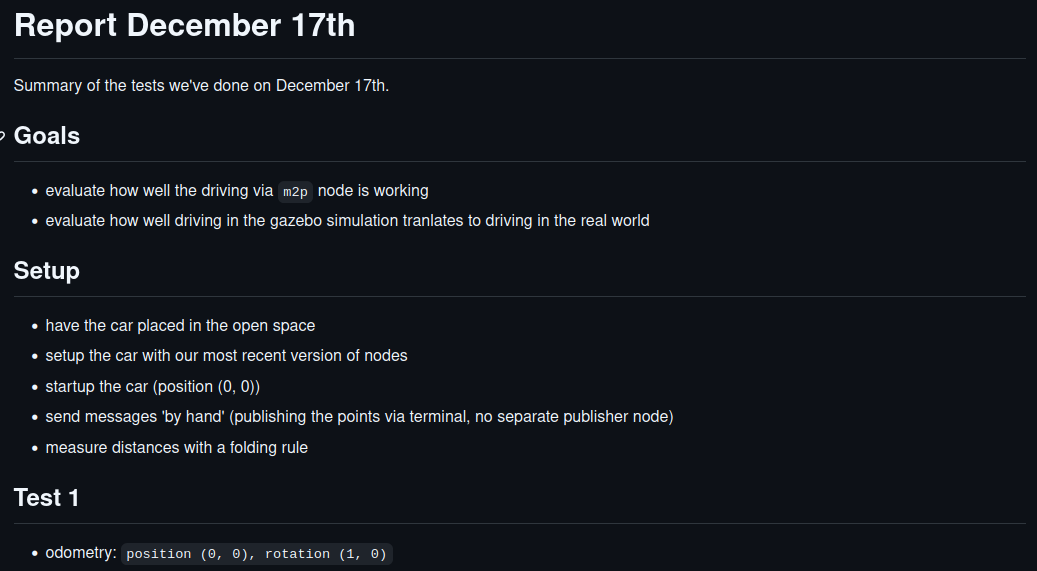
\includegraphics[width=\columnwidth]{protocol.png}}
		\caption{Screenshot of a test report.}
		\label{fig:protocol}
	\end{center}
	\vskip -0.2in
\end{figure}


\section{Challenges}
During the development of the project the team faced multiple challenges. The core problem of the project was the translation of the car's behavior from the simulation into the real world. The following challenges required a lot of time to handle and overcome, which resulted in unexpected developmental delays.\\
\newline
Whilst working on the M2P node and working on the validation in the real world we had to find out, that ROS and Gazebo use different coordinate systems, which resulted in correct calculations in the simulations yet incorrect ones in real world testing. This was due to the odometry and the target points not adhering to the same coordinate system. This problem was overcome by writing a transform node which would translate between both coordinate systems depending on the usage context. 
Additionally, during a debugging session it occurred that there was another difference between simulation and real world. In the real world scenario, the racecar would stop just before the range for the M2P node to consider a point to be reached. This was due to a too small velocity in the drive message for the racecar to move forward. To overcome this issue, a minimum velocity was implemented and the handling of target points in the M2P node was adjusted slightly.\\
\newline
Furthermore the team encountered problems with the transform tree and working with the rosbags. These problems have expressed themselves in a heavily drifting odometry and lookup errors for sensor data. With these issues self-localization and mapping seemed impossible in a real world scenario. Fortunately, after a system update on the racecar the problem was solved and the racecar was driving in the ROS coordinate system.


\section{Outcomes}

Following for implementation and after facing the challenges, we have a race car that can drive autonomously in simulation \href{https://www.youtube.com/watch?v=qzKs0KKohVE&ab_channel=Ossmos}{(watch this video)}. In the real world setting, we are still facing issues with the perception, since the car still cannot reliably classify cones by the color. This makes it impossible for the car to successfully maneuver in turns as soon as there are cones of one color (blue or yellow) missing for the calculation of the next target point. \\ \newline
Based on the dependencies between requirements and an initial prioritization  only a subset of the requirements was fulfilled. These requirements include F01 - F04, F06, F09 - F11, F14 - F16, F20 - F23, F28, F31, F34. Q11, Q16, Q19, C01, C02, and C07 - C11. Still, there are some requirements that were realized in a way that we did not initially plan for it. These include F14, where the vehicle stops driving since it is uncertain of the next target point because of missing cone classifications. Yet, in our current implementation, we do not check whether the car is still on the track or not. For Q19 we filter the data during our sensor fusion and cluster detection, rejecting clusters, that do not fit the dimensions of a cone. Finally, while the vehicle was tested on track as described in C08 and F34, those tests were not successful. \\
\newline
During development our understanding of the stack and our solution space has changed, which also yields a change in requirements. The following table displays the subset of the changed requirements which in this form can be considered as done. \\

\begin{center}
	\begin{longtable}{ | m{2em} | m{10em} | m{16em} | m{8em} | }
		\caption{Changed Requirements.} \label{tab:long}\\
		
		\hline \multicolumn{1}{|m{2em}|}{\textbf{ID}} & \multicolumn{1}{m{10em}|}{\textbf{Requirement Name}} & \multicolumn{1}{m{16em}|}{\textbf{Requirement}} & \multicolumn{1}{m{8em}|}{\textbf{Classification}} \\ \hline
		\endfirsthead
		
		\multicolumn{4}{m{36em}}%
		{{\bfseries \tablename\ \thetable{} -- continued from previous page}} \\
		\hline \multicolumn{1}{|m{2em}|}{\textbf{ID}} & \multicolumn{1}{m{10em}|}{\textbf{Requirement Name}} & \multicolumn{1}{m{16em}|}{\textbf{Requirement}} & \multicolumn{1}{m{8em}|}{\textbf{Classification}} \\ \hline
		\endhead
		
		\hline \multicolumn{4}{|m{36em}|}{Continued on next page} \\ \hline
		\endfoot
		
		\hline \hline
		\endlastfoot
		
		F08* & Self-Localization & The vehicle shall localize itself relative to a map using fused data from LiDAR, camera, and odometry. & Must have \\ \hline
		F12* & Path Planning & The vehicle shall employ a path planning algorithm that plans a static path after an exploration lap. & Must have \\ \hline
		Q02* & Control Loop Frequency & The vehicle shall maintain a control loop update frequency of ca. 5 HZ to ensure smooth and responsive at ca. 1 m/s. & Must have \\ \hline
		Q04* & Perception Radius & The perception system shall detect cones within the range of the sensor overlap (LiDAR and camera) to provide sufficient time for target point calculations. & Must have \\ \hline
		C03* & Real-Time Performance & The system shall process sensor inputs at ca. 5 Hz to maintain real-time performance within the computational limits of the vehicle. & Must have \\ \hline
		C04* & Remote Emergency Stop & The vehicle shall include a Remote Emergency Stop that can be triggered by the race team at any time. & Must have
	\end{longtable}
\end{center}

Lastly, there are still requirements left, that were not (fully) fulfilled since they were outside our time scope, became obsolete due to our approach, or are currently technically unfulfillable.
\begin{itemize}
	\item F05: As we calculate the target point in our exploration phase as the midpoint between the closest blue and yellow cones in driving distance, we assume that we stay within track boundaries with this approach and the continuous estimation of the distance to the track boundaries becomes obsolete.
	\item F13, Q20: This is obsolete since the track layout doesn't change during race and path planning only happens after track is fully explored. 
	\item F17: For our speeds it is not quite necessary to adapt the acceleration with regards of factors like friction, currently the acceleration is adjusted by distance to next target point and the maximum speed is managed with an adjustable parameter.
	\item F18: The handling is not yet implemented as it is not needed at low speeds (at least in simulation).
	\item F19: The smooth acceleration not really possible with the current acceleration mode of car at low speeds. The acceleration is per default jerky at low speeds.
	\item F24: We did not focus on smooth steering exclusively since at current maximum speeds of around 1 m/s the steering did not require any improvement in that regard.
	\item F25, F32, Q06, C12: Currently we handle emergency stops and breaking by manually killing the nodes. There is yet no behavior implemented for detecting and handling emergency situations. For these reasons an override mode for emergency cases seems obsolete.
	\item F26, F27, F29, F30, F33, Q09, Q10, Q12, Q13, C05, C06, C12: Currently nodes can crash independently. Since our nodes are dependent on the messages from other nodes which are handled in callbacks and a crashed node does not send messages, at some point the vehicle will stop driving as it is not receiving any new target point. With the current connection it is not possible to retrieve any system health data, as it will just overload the connection. Still, there are logs for nodes and it is detectable when a node runs into an error and crashes. One still might investigate into an autonomous restart of a node after node failure.
	\item Q01: Similarly to the system health the latency of the sensor processing cannot be tracked in current state.
	\item Q03: Currently, we have found no way to validate the localization accuracy.
	\item Q08: Currently, we cannot determine a certain threshold at which cones must be classified. Additionally, the classification range varies between simulation and real world.
	\item Q14: At the current state, the perception algorithms do not have ROS2 parameters. It is still to evaluate which benefit a reconfiguration of algorithmic parameters during runtime would yield in contrast to restarting the node (stack) entirely with changed parameters.
	\item Q17: During our implementation, we did not run into any energy consumption problems that would require acute improvements.
	\item Q18: While setting the sensor frequency or the frequency of callbacks does not happen autonomously, we have set these frequencies accordingly for our current maximum speed.
\end{itemize}

\section{Reflection}
\textbf{TODO: Review wheter not met requirements can be implemented with the current stack.}
Looking back on the expectations to this project and the faced challenges during development, it is clear that not every requirement could be fulfilled with the given time constraints. While the racecar is able to execute basic autonomous driving tasks like cone detection and classification, self-localization, path planning, and map generation, some requirements that fall under the category ``could have'' were not realized.\\
\newline
These requirements were for example the emergency braking, failsafe mode, or the health monitoring. These were partially not implemented due to a lower priority. While the racecar does not register driving failures like leaving the track by itself, quitting the nodes does result in an immediate stop since the racecar does not receive any more drive messages. This resulted in the emergency stop to be obsolete for the current state. Due to the time constraints there is no guarantee on the quality requirements. \\
\newline
In further development, one could review the existing requirements - especially under the factor of actually achieved top speeds during the race - and adjust them. The optional requirements that were not fulfilled could be reviewed under the point on necessity and implemented given a prioritization. \\
\newline
\textbf{TODO: What could be changed in the development process, the tech stack, etc. for further improvement and for future iterations of the course?}
\subsection{Possible Changes for the next Course Iteration}
For the next iteration of the course, several key improvements could enhance the learning experience and the performance of the autonomous vehicle. First, providing more structured guidance on handling ROS2 and debugging techniques is expected to facilitate participants in overcoming technical hurdles in a more efficient way.
Additionally, improving the internet connection to the car by implementing a more resilient WiFi network will ensure smoother data transfer and reduce connection drops, which currently hinder real-time operation.\\
From a performance perspective, the refinement of the vehicle's driving capabilities at lower speeds with finer acceleration control will improve maneuverability and precision. 
Furthermore, upgrading the camera to a model with a wider field of view (120°–140°) and repositioning it centrally rather than its current left-leaning placement will enhance perception and environmental awareness. 
Finally, the consideration of a Raspberry Pi-based vehicle as an alternative platform has the potential to offer a cost-effective solution while retaining the essential functionalities of the system.

% Here we could come back to the expectations and discuss why we did not do some parts

\newpage

\bibliographystyle{alpha}
\bibliography{bibliography}

\end{document}
